%\begin{noindent}
\begin{markdown}
# Kabel

## Allgemeines

\begin{wrapfigure}{r}{0.5\textwidth}
    \vspace{-1em}
    \centering
    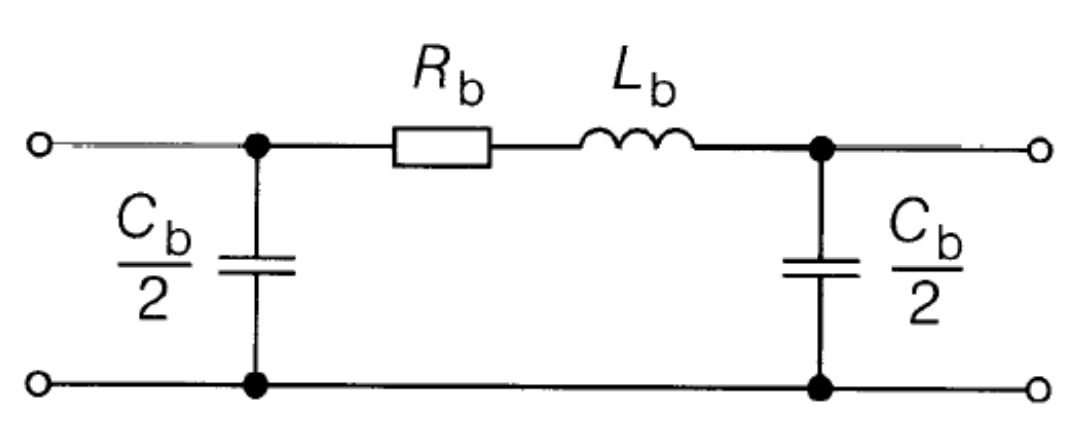
\includegraphics[width=0.4\textwidth]{./images/09-Kabel/Ersatzschaltbild.png}
    \caption[Ersatzschaltbild eines Kables]{Ersatzschaltbild eines Kables}
\end{wrapfigure}

Es wird zwischen folgenden Kabelarten unterschieden:

- Niederspannung
- Mittelspannung
- Einadrig
- Hochspannung
    - Gasaußendruck
    - Gasinnendruck

### Typenbezeichnung

\begin{wrapfigure}{r}{0.5\textwidth}
    \centering
    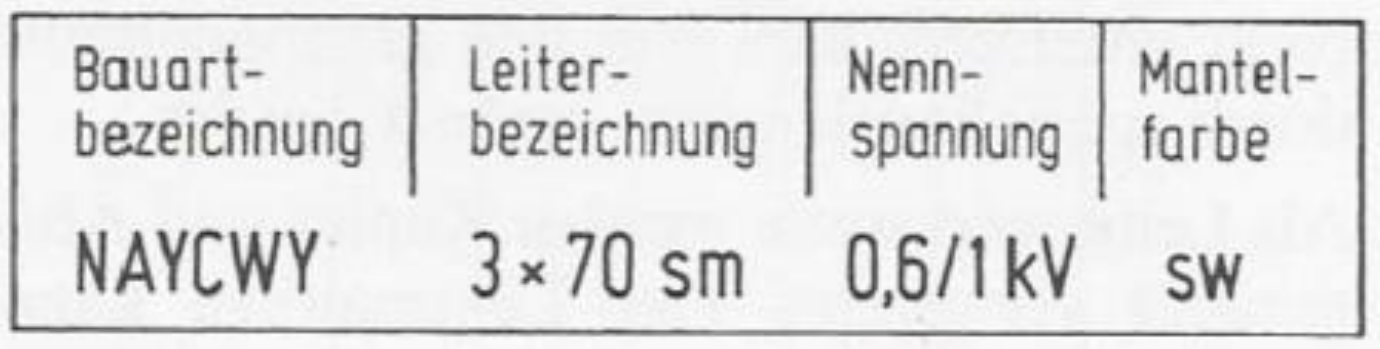
\includegraphics[width=0.4\textwidth]{./images/09-Kabel/Typenbezeichnung.png}
    \caption[Typenbezeichnung eines Kables]{Typenbezeichnung eines Kables}
\end{wrapfigure}

Folgende Informationen können aus der Typenbezeichnung entnommen werden:

- Aufbau
- Aderzahl
- Leiterquerschnitt
- Leiterform
- Nennspannung
- Farbe des Außenmantels

### Kostenvergleich

\GrayBox{Erdkabel sind 2 bis 5-mal teurer als Freileitungen.}

Beim Erdkabel muss die **kapazitive Blindleistung alle 30 bis 40 km kompensiert** werden. _(Es muss an die Oberfläche geführt werden)_

Daher muss eine Analyse durchgeführt werden, ob der Einsatz von Erdkabeln möglich ist.

### Zulässige Betriebsströme

\GrayBox{Die einzelnen Bemessungsströme für verschiedene Kabelbauarten sind in der Norm angegeben. _(DIN VDE 0276)_}

Mit zunehmender Erwärmung verkürzt sich die Lebensdauer (da sich der Verlustfaktor erhöht).
Die Temperatur ist abhängig von:

- Verlegungsart _(Bündel oder nebeneinander)_
- Umgebungstemperatur
- Wärmeableitung
- Lastverlauf
- Anzahl der parallel verlegten Systeme

\end{markdown}

Der Lastverlauf wird mit Belastungsgrad $B$ definiert. ($B = \frac{P_{Mittelwert}}{P_{Max}}$)

\begin{align*}
    B &= 1   & \text{Dauerlast}\\
    B &= 0,7 & \text{EVU-Last} 
\end{align*}

%\begin{noindent}
\begin{markdown}

Bei luftverlegten Kabeln wird die Dauerlast _(B=1)_ als Standard angenommen, ber Erdkabeln die EVU-Last.

\newpage

## Niederspannungskabel

PVC-isolierte Starkstromkabel sind **ein- und mehradrig in Verwendung**

**Verwendung:** _(keine nachträgliche Beschädigungen wird erwartet)_

- Kabelkanälen
- Innenräume
- im Freien
- im Wasser
- in Erde

\begin{wrapfigure}{r}{0.5\textwidth}
    \centering
    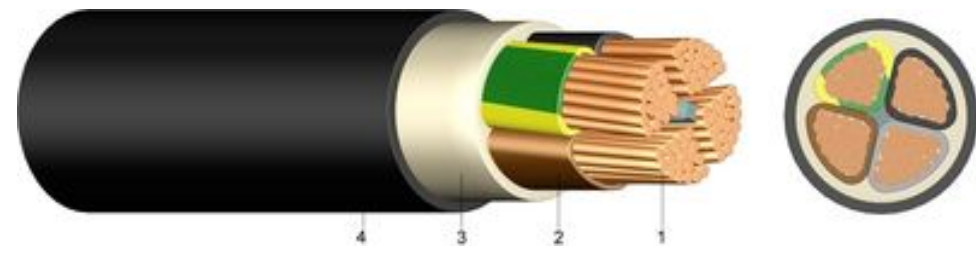
\includegraphics[width=0.4\textwidth]{./images/09-Kabel/Niederspannungskabel.png}
    \caption[Niederspannungskabel]{Niederspannungskabel}
\end{wrapfigure}

**Aufbau:**

#. Kupferleiter (blank-, ein- oder mehrdrähtig)
#. Aderisolation (PVC)
#. FüllMantel (PVC)
#. Außenmantel (PVC, schwarz)

## Mittelspannungskabel

**Verwendung:** _(Industrie- und Schaltanlagen)_

- Kabelkanälen
- Innenräume
- im Freien
- in Erde

\begin{wrapfigure}{r}{0.6\textwidth}
    \centering
    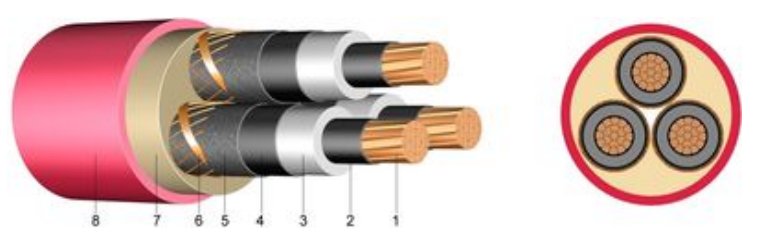
\includegraphics[width=0.5\textwidth]{./images/09-Kabel/Mittelspannungskabel.png}
    \caption[Mittelspannungskabel]{Mittelspannungskabel}
\end{wrapfigure}

**Aufbau:**

#. Kupferleiter (blank oder mehrdrähtig)
#. Innere Leiterschicht
#. Aderisolation (VPE)
#. Äußere Leiterschicht
#. Leitendes Band
#. Abschirmung
#. Füllmantel
#. Außenmantel (PVC, rot)

Die Leiterformen werden so gewählt, dass der Kabelquerschnitt gut ausgenutzt wird. 

Kabel werden zum Schutz gegen Feuchtigkeit, mechanische und chemische Einflüsse mit einem Schutzmantel versehen. _(meist aus PVC, Blei oder Aluminium)_

Um bei Spannungen über 6kV, die hohe Beanspruchung des elektrischen Feldes zu verringern, wird eine leitende Schicht zwischen den Leitern und der Aderisolierung aufgetragen. _(Ansonsten kann es zu einem Durchschlag der Isolierung kommen)_

\begin{figure}[H]
    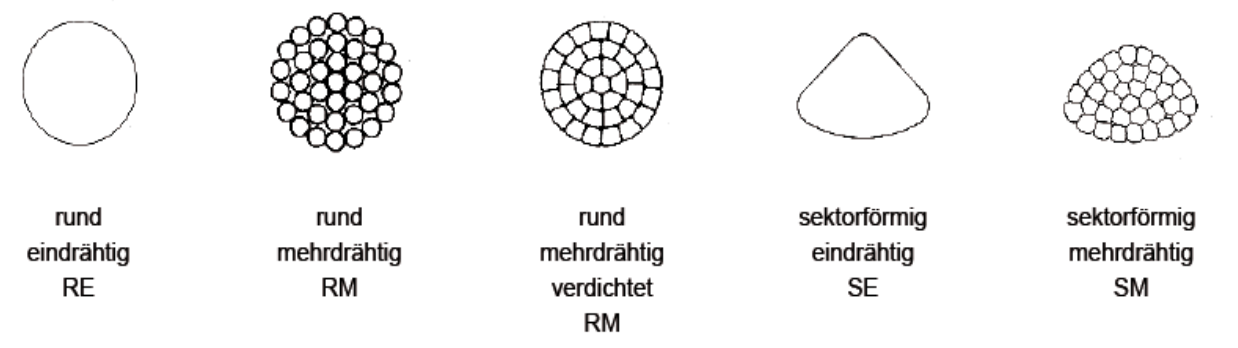
\includegraphics[width=\linewidth]{./images/09-Kabel/Mittelspannungskabel-Leiterformen.png}
    \caption[Leiterformen von Mittelspannungskabel]{Leiterformen von Mittelspannungskabel}
\end{figure}

\newpage

## Einadrige Kabel

**Vorteile:** _(gegenüber dreiadrige Kabel)_

- größere Lieferlängen
- hohe Strombelastbarkeit
- größere Biegsamkeit
- geringeres Gewicht 

**Nachteile:**

- Benötigen beim nebeneinander Verlegen mehr Platz 
- Heben ihre Magnetfelder nicht auf _(bilden unsymmetrische Systeme)_
    - müssen deshalb zyklisch vertauscht werden 

**Aufbau:**

#. Kupferleiter (mehradrig, rund)
#. Innere Leiterschicht
#. Aderisolation
#. Äußere Leiterschicht
#. Abschirmung
#. Außenmantel

\begin{figure}[H]
    \centering
    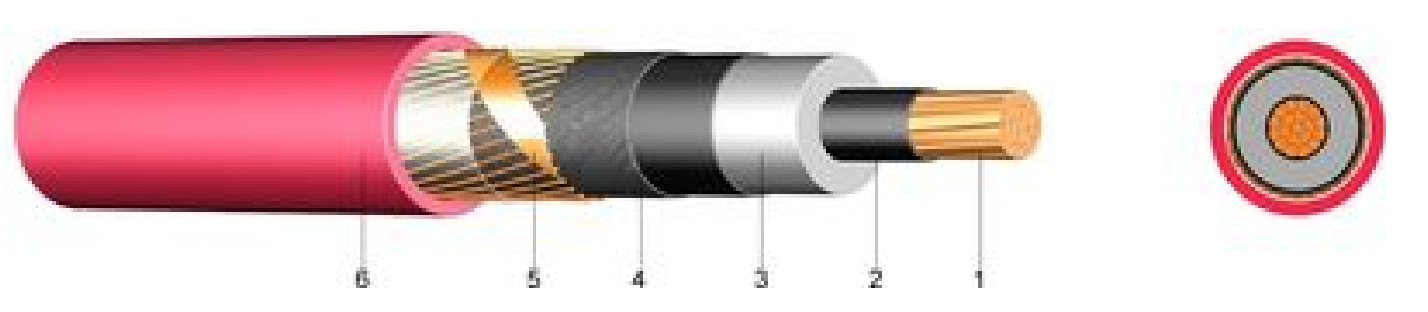
\includegraphics[width=0.8\textwidth]{./images/09-Kabel/Einzeladerkabel.png}
    \caption[Einzeladerkabel]{Einzeladerkabel}
\end{figure}

## Hochspannungskabel

\GrayBox{Für Spannungen über 60 kV wird die Aderisolierung unter Öl- oder Gasdruck gesetzt. _(Um Streuungen des elektrischen Feldes zu vermeiden)_}

### Gasaußendruckkabel

**Aufbau:**

#. Kupferleiter
#. Papierisolierung
#. Bleimantel
#. Druckschutzbandage
#. Verseilung der Kabeladern
#. Verstärkung aus Stahlflachdrähten
#. Stahlrohr
#. Umhüllung

### Gasinnendruckkabel

**Aufbau:**

#. Kupferleiter
#. Papierisolierung
#. Verseilung der Kabeladern
#. Verstärkung aus Stahlflachdrähten
#. Stahlrohr
#. Umhüllung

\end{markdown}